\tableofcontents
\section{UnitType}
\subsection{接口类}
\subsection{BWAPI::UnitType继承图}
\begin{figure}[H]
    \centering
    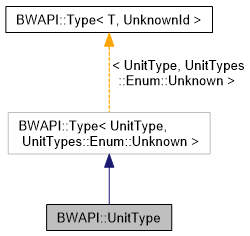
\includegraphics[width=0.4\textwidth]{figures/UnitType继承图.png}
\end{figure}
\subsubsection{公共成员函数}
\begin{codebox}[公共成员函数]
constexpr UnitType (int id=UnitTypes::Enum::None)
const SetContainer< TechType > & abilities () const
int acceleration () const
WeaponType airWeapon () const
int armor () const
UpgradeType armorUpgrade () const
int buildScore () const
const UnitType::set & buildsWhat () const
\end{codebox}
\begin{codebox}[公共成员函数]
int buildTime () const
bool canAttack () const
bool canBuildAddon () const
bool canMove () const
bool canProduce () const
TechType cloakingTech () const
int destroyScore () const
int dimensionDown () const
int dimensionLeft () const
int dimensionRight () const
int dimensionUp () const
int gasPrice () const
Race getRace () const
WeaponType groundWeapon () const
int haltDistance () const
bool hasPermanentCloak () const
int height () const
bool isAddon () const
bool isBeacon () const
bool isBuilding () const
bool isBurrowable () const
bool isCloakable () const
bool isCritter () const
bool isDetector () const
bool isFlagBeacon () const
bool isFlyer () const
bool isFlyingBuilding () const
bool isHero () const
bool isInvincible () const
bool isMechanical () const
bool isMineralField () const
bool isNeutral () const
\end{codebox}
\begin{codebox}[公共成员函数]
bool isOrganic () const
bool isPowerup () const
bool isRefinery () const
bool isResourceContainer () const
bool isResourceDepot () const
bool isRobotic () const
bool isSpecialBuilding () const
bool isSpell () const
bool isSpellcaster () const
bool isSuccessorOf (UnitType type) const
bool isTwoUnitsInOneEgg () const
bool isWorker () const
int maxAirHits () const
int maxEnergy () const
int maxGroundHits () const
int maxHitPoints () const
int maxShields () const
int mineralPrice () const
bool producesCreep () const
bool producesLarva () const
bool regeneratesHP () const
TechType requiredTech () const
const std::map< UnitType, int > & requiredUnits () const
bool requiresCreep () const
bool requiresPsi () const
const SetContainer< TechType > & researchesWhat () const
int seekRange () const
int sightRange () const
UnitSizeType size () const
\end{codebox}
\begin{codebox}[公共成员函数]
int spaceProvided () const
int spaceRequired () const
int supplyProvided () const
int supplyRequired () const
int tileHeight () const
TilePosition tileSize () const
int tileWidth () const
double topSpeed () const
int turnRadius () const
const SetContainer< UpgradeType > & upgrades () const
const SetContainer< UpgradeType > & upgradesWhat () const
const std::pair< UnitType, int > whatBuilds () const
int width () const
\end{codebox}
\subsubsection{详细描述}
UnitType 类用于获取特定unit类型的信息,例如unit的成本(cost)、建造时间(build time)、武器(weapon)、生命值(hit points)、能力(abilities)等。
\begin{refer}
\begin{itemize}
    \item UnitInterface::getType
    \item UnitTypes
\end{itemize}
\end{refer}
\subsubsection{构造函数\&析构函数文档}
\begin{tcolorbox}[colback=white, colframe=black!60!white, title=UnitType(), arc=0mm]
    \begin{minted}[frame=none]{cpp}
constexpr BWAPI::UnitType::UnitType (int id = UnitTypes::Enum::None)
    \end{minted}
预期类型构造函数\par
如果type是无效类型(invalid type),则会变成   Types::Unknown  。如果type的值小于 0 或大于   Types::Unknown  ,则该type无效
\begin{parameter}
\begin{itemize}
    \item id:与该type对应的 ID。它通常是一个整数值,对应于 Broodwar 的内部类型。如果给定的 ID 无效,则会变成   Types::Unknown  。
\end{itemize}
\end{parameter}
\end{tcolorbox}

\subsubsection{成员函数文档}

\begin{tcolorbox}[colback=white, colframe=black!60!white, title=abilities(), arc=0mm]
    \begin{minted}[frame=none]{cpp}
const SetContainer<TechType>& BWAPI::UnitType::abilities () const
    \end{minted}
检索此Unit在游戏中可用的技能集合。
\begin{return}
\begin{itemize}
    \item SetContainer<TechType>:包含技能信息的   TechTypes   集合。
\end{itemize}
\end{return}
\end{tcolorbox}


\begin{tcolorbox}[colback=white, colframe=black!60!white, title=acceleration(), arc=0mm]
    \begin{minted}[frame=none]{cpp}
int BWAPI::UnitType::acceleration () const
    \end{minted}
检索unit的加速度。
\begin{return}
\begin{itemize}
    \item int:unit达到最高速度的加速度。
\end{itemize}
\end{return}
\end{tcolorbox}

\begin{tcolorbox}[colback=white, colframe=black!60!white, title=airWeapon(), arc=0mm]
    \begin{minted}[frame=none]{cpp}
WeaponType BWAPI::UnitType::airWeapon () const
    \end{minted}
检索此UnitType的对空WeaponType。
\begin{return}
\begin{itemize}
    \item WeaponType:此UnitType用于攻击空中目标的Weapontype。
\end{itemize}
\end{return}
\end{tcolorbox}


\begin{tcolorbox}[colback=white, colframe=black!60!white, title=armor(), arc=0mm]
    \begin{minted}[frame=none]{cpp}
int BWAPI::UnitType::armor () const
    \end{minted}
检索该UnitType初始的默认护甲值,不包括任何升级。
\begin{note}
此值可能与Use Map Settings游戏类型中看到的值不一致。
\end{note}
\begin{return}
\begin{itemize}
    \item int:UnitType所拥有的护甲值。
\end{itemize}
\end{return}
\end{tcolorbox}


\begin{tcolorbox}[colback=white, colframe=black!60!white, title=armorUpgrade(), arc=0mm]
    \begin{minted}[frame=none]{cpp}
UpgradeType BWAPI::UnitType::armorUpgrade () const
    \end{minted}
检索用于增加此UnitType护甲的升级类型(UpgradeType)\par
每次升级,此UnitType会获得 +1 的额外护甲。
\begin{return}
\begin{itemize}
    \item UpgradeType:表示增加此UnitType护甲数量的升级类型。
\end{itemize}
\end{return}
\end{tcolorbox}


\begin{tcolorbox}[colback=white, colframe=black!60!white, title=buildScore(), arc=0mm]
    \begin{minted}[frame=none]{cpp}
int BWAPI::UnitType::buildScore () const
    \end{minted}
检索建造此UnitType所获得的分数。\par
此值用于计算游戏结束后的得分屏幕上的分数。
\begin{return}
\begin{itemize}
    \item int:建造此UnitType所获得的分数。
\end{itemize}
\end{return}
\end{tcolorbox}


\begin{tcolorbox}[colback=white, colframe=black!60!white, title=buildsWhat(), arc=0mm]
    \begin{minted}[frame=none]{cpp}
const UnitType::set& BWAPI::UnitType::buildsWhat () const
    \end{minted}
    检索此UnitType能够创建的unit集合。\par
    这包括训练、建造、传送和变形。
\begin{note}
    某些地图有特殊参数,可能会禁用通常可以建造的unit。可以使用   PlayerInterface::isUnitAvailable   来确定某个UnitType是否在当前游戏中对特定player可用。
\end{note}
\begin{return}
\begin{itemize}
    \item UnitType::set:包含此UnitType可以建造的unit。
\end{itemize}
\end{return}
\begin{refer}
\begin{itemize}
    \item PlayerInterface::isUnitAvailable  :用于判断某个UnitType是否对特定player可用。
\end{itemize}
\end{refer}
\end{tcolorbox}


\begin{tcolorbox}[colback=white, colframe=black!60!white, title=buildTime(), arc=0mm]
    \begin{minted}[frame=none]{cpp}
int BWAPI::UnitType::buildTime () const
    \end{minted}
    检索训练、变形或建造该unit所需的默认时间,以frame为单位。
\begin{note}
    此值可能与 Use Map Settings 游戏类型中显示的值不一致。
\end{note}
\begin{return}
\begin{itemize}
    \item int:建造该unit所需的frame数。
\end{itemize}
\end{return}
\begin{refer}
\begin{itemize}
    \item UnitInterface::getRemainingBuildTime  :用于获取unit剩余的建造时间。
\end{itemize}
\end{refer}
\end{tcolorbox}


\begin{tcolorbox}[colback=white, colframe=black!60!white, title=canAttack(), arc=0mm]
    \begin{minted}[frame=none]{cpp}
bool BWAPI::UnitType::canAttack () const
    \end{minted}
    检查该unit是否能够进行攻击。
\begin{note}
    对于只能通过特殊技能造成伤害的unit(例如高阶圣堂武士),此函数将返回   false
\end{note}
\begin{return}
\begin{itemize}
    \item bool:如果该UnitType能够通过标准攻击对其他unit造成伤害,则返回   true  ,否则返回   false
\end{itemize}
\end{return}
\end{tcolorbox}


\begin{tcolorbox}[colback=white, colframe=black!60!white, title=canBuildAddon(), arc=0mm]
    \begin{minted}[frame=none]{cpp}
bool BWAPI::UnitType::canBuildAddon () const
    \end{minted}
    检查该UnitType是否能够建造附加建筑。
\begin{return}
\begin{itemize}
    \item bool:如果该UnitType能够建造附加建筑,则返回   true  ,否则返回   false  。
\end{itemize}
\end{return}
\begin{refer}
\begin{itemize}
    \item isAddon  :用于检查某个UnitType是否能附加建筑。
\end{itemize}
\end{refer}
\end{tcolorbox}


\begin{tcolorbox}[colback=white, colframe=black!60!white, title=canMove(), arc=0mm]
    \begin{minted}[frame=none]{cpp}
bool BWAPI::UnitType::canMove () const
    \end{minted}
    检查该UnitType是否能够移动。
\begin{note}
    建筑物将返回   false  ,包括升起时能够移动的 Terran 可升降建筑。
\end{note}
\begin{return}
\begin{itemize}
    \item bool:如果该unit能够使用移动命令,则返回   true  ,否则返回   false
\end{itemize}
\end{return}
\end{tcolorbox}


\begin{tcolorbox}[colback=white, colframe=black!60!white, title=canProduce(), arc=0mm]
    \begin{minted}[frame=none]{cpp}
bool BWAPI::UnitType::canProduce () const
    \end{minted}
    确定一个单位是否能够生产其他单位。\par
    例如\verb|Terran_Barracks.canProduce()|将返回true,而\verb|Terran_Marine.canProduce()|将返回   false  。
    这同样适用于两种非建筑单位:航空母舰(Carrier)可以生产拦截机(interceptors)和雷兽(Reaver)可以生产甲虫(scarabs)
\begin{return}
\begin{itemize}
    \item bool:如果该unit能够使用移动命令,则返回   true  ,否则返回   false
\end{itemize}
\end{return}
\end{tcolorbox}


\begin{tcolorbox}[colback=white, colframe=black!60!white, title=cloakingTech(), arc=0mm]
    \begin{minted}[frame=none]{cpp}
TechType BWAPI::UnitType::cloakingTech () const
    \end{minted}
    检索与某些unit相关的隐形技术。
\begin{return}
\begin{itemize}
    \item TechType:表示该UnitType使用的隐形技术作为能力。\par
    (TechTypes::None  :如果该UnitType没有主动隐形能力。)
\end{itemize}
\end{return}
\end{tcolorbox}


\begin{tcolorbox}[colback=white, colframe=black!60!white, title=destroyScore(), arc=0mm]
    \begin{minted}[frame=none]{cpp}
int BWAPI::UnitType::destroyScore () const
    \end{minted}
    检索击杀该UnitType所获得的分数。\par
    此值用于计算游戏结束后的得分屏幕上的分数。
\begin{return}
\begin{itemize}
    \item int:击杀该UnitType所获得的分数。
\end{itemize}
\end{return}
\begin{refer}
    \begin{itemize}
        \item buildScore:建造该UnitType所获得的分数。
    \end{itemize}
\end{refer}
\end{tcolorbox}


\begin{tcolorbox}[colback=white, colframe=black!60!white, title=dimensionDown(), arc=0mm]
    \begin{minted}[frame=none]{cpp}
int BWAPI::UnitType::dimensionDown () const
    \end{minted}
    检索UnitType中心到其下边缘的距离。
\begin{return}
\begin{itemize}
    \item int:从UnitType中心到其下边缘的距离,以pixel为单位。。
\end{itemize}
\end{return}
\end{tcolorbox}


\begin{tcolorbox}[colback=white, colframe=black!60!white, title=dimensionLeft(), arc=0mm]
    \begin{minted}[frame=none]{cpp}
int BWAPI::UnitType::dimensionLeft () const
    \end{minted}
    检索UnitType中心到其左边缘的距离。
\begin{return}
\begin{itemize}
    \item int:从UnitType中心到其左边缘的距离,以pixel为单位。
\end{itemize}
\end{return}
\end{tcolorbox}


\begin{tcolorbox}[colback=white, colframe=black!60!white, title=dimensionRight(), arc=0mm]
    \begin{minted}[frame=none]{cpp}
int BWAPI::UnitType::dimensionRight () const
    \end{minted}
    检索UnitType中心到其右边缘的距离。
\begin{return}
\begin{itemize}
    \item int:从UnitType中心到其右边缘的距离,以pixel为单位。
\end{itemize}
\end{return}
\end{tcolorbox}


\begin{tcolorbox}[colback=white, colframe=black!60!white, title=dimensionUp(), arc=0mm]
    \begin{minted}[frame=none]{cpp}
int BWAPI::UnitType::dimensionUp () const
    \end{minted}
    检索UnitType中心到其上边缘的距离。
\begin{return}
\begin{itemize}
    \item int:从UnitType中心到其上边缘的距离,以pixel为单位。
\end{itemize}
\end{return}
\end{tcolorbox}


\begin{tcolorbox}[colback=white, colframe=black!60!white, title=gasPrice(), arc=0mm]
    \begin{minted}[frame=none]{cpp}
int BWAPI::UnitType::gasPrice () const
    \end{minted}
    检索购买该unit的默认瓦斯(Vespene Gas)价格。
\begin{note}
    此值可能与“使用地图设置”游戏类型中显示的值不一致。
\end{note}
\begin{return}
\begin{itemize}
    \item int:该unit的瓦斯成本。
\end{itemize}
\end{return}
\end{tcolorbox}


\begin{tcolorbox}[colback=white, colframe=black!60!white, title=gasPrice(), arc=0mm]
    \begin{minted}[frame=none]{cpp}
int BWAPI::UnitType::gasPrice () const
    \end{minted}
    检索购买该unit的默认瓦斯(Vespene Gas)价格。
\begin{note}
    此值可能与“使用地图设置”游戏类型中显示的值不一致。
\end{note}
\begin{return}
\begin{itemize}
    \item int:该unit的瓦斯成本。
\end{itemize}
\end{return}
\end{tcolorbox}


\begin{tcolorbox}[colback=white, colframe=black!60!white, title=getRace(), arc=0mm]
    \begin{minted}[frame=none]{cpp}
Race BWAPI::UnitType::getRace () const
    \end{minted}
    检索该UnitType所属的种族。
\begin{return}
\begin{itemize}
    \item Race:表示拥有该UnitType的种族。\par (Race::None:表示该UnitType不属于任何特定种族(例如中立生物)。)
\end{itemize}
\end{return}
\end{tcolorbox}


\begin{tcolorbox}[colback=white, colframe=black!60!white, title=groundWeapon(), arc=0mm]
    \begin{minted}[frame=none]{cpp}
WeaponType BWAPI::UnitType::groundWeapon () const
    \end{minted}
    检索该UnitType用于攻击地面目标的WeaponType。
\begin{return}
\begin{itemize}
    \item WeaponType:该UnitType用于地面攻击的   WeaponType 
\end{itemize}
\end{return}
\end{tcolorbox}


\begin{tcolorbox}[colback=white, colframe=black!60!white, title=haltDistance(), arc=0mm]
    \begin{minted}[frame=none]{cpp}
int BWAPI::UnitType::haltDistance () const
    \end{minted}
    检索unit的停止距离。\par 这决定了unit停止移动的速度。
\begin{return}
\begin{itemize}
    \item int:unit的停止距离值。
\end{itemize}
\end{return}
\end{tcolorbox}


\begin{tcolorbox}[colback=white, colframe=black!60!white, title=hasPermanentCloak(), arc=0mm]
    \begin{minted}[frame=none]{cpp}
bool BWAPI::UnitType::hasPermanentCloak () const
    \end{minted}
    检查该UnitType是否始终处于隐形状态。\par 这意味着该UnitType始终处于隐形状态,需要Detector才能看到它。
\begin{return}
\begin{itemize}
    \item bool:如果该UnitType始终处于隐形状态,则返回   true  ,否则返回   false  。
\end{itemize}
\end{return}
\end{tcolorbox}


\begin{tcolorbox}[colback=white, colframe=black!60!white, title=height(), arc=0mm]
    \begin{minted}[frame=none]{cpp}
int BWAPI::UnitType::height () const
    \end{minted}
    用于检索UnitType高度的宏,其高度通过   dimensionUp + dimensionDown + 1   计算得出。
\begin{return}
\begin{itemize}
    \item int:unit的高度,以pixel为单位。
\end{itemize}
\end{return}
\end{tcolorbox}


\begin{tcolorbox}[colback=white, colframe=black!60!white, title=isAddon(), arc=0mm]
    \begin{minted}[frame=none]{cpp}
bool BWAPI::UnitType::isAddon () const
    \end{minted}
    检查该unit是否是附加建筑。\par 附加建筑是某些人类建筑的扩展部分,例如通讯卫星站(Comsat Station)。
\begin{return}
\begin{itemize}
    \item bool:如果该unit是附加建筑,则返回   true  ,否则返回   false  。
\end{itemize}
\end{return}
\begin{note}
    如果此函数返回成功状态,则以下函数调用也将返回成功状态:
    \begin{itemize}
        \item getRace() == Races::Terran  (该单位属于人类种族)
        \item isBuilding()  (该单位是建筑)
    \end{itemize}
\end{note}
\end{tcolorbox}


\begin{tcolorbox}[colback=white, colframe=black!60!white, title=isBeacon(), arc=0mm]
    \begin{minted}[frame=none]{cpp}
bool BWAPI::UnitType::isBeacon () const
    \end{minted}
    每个种族都有一个信标,分别是   \verb|UnitTypes::Special_Zerg_Beacon|  (虫族信标)、  \verb|UnitTypes::Special_Terran_Beacon|  (人类信标)和   \verb|UnitTypes::Special_Protoss_Beacon|  (神族信标)。
\begin{refer}
    \begin{itemize}
        \item  isFlagBeacon:用于检查单位是否是旗帜信标。
    \end{itemize}
\end{refer}
\begin{return}
\begin{itemize}
    \item bool:如果该UnitType是三个种族信标之一,则返回   true  ,否则返回   false  。
\end{itemize}
\end{return}
\end{tcolorbox}


\begin{tcolorbox}[colback=white, colframe=black!60!white, title=isBuilding(), arc=0mm]
    \begin{minted}[frame=none]{cpp}
bool BWAPI::UnitType::isBuilding () const
    \end{minted}
\begin{return}
\begin{itemize}
    \item bool:如果该单位是建筑,则返回   true  ,否则返回   false  。
\end{itemize}
\end{return}
\end{tcolorbox}


\begin{tcolorbox}[colback=white, colframe=black!60!white, title=isBurrowable(), arc=0mm]
    \begin{minted}[frame=none]{cpp}
bool BWAPI::UnitType::isBurrowable () const
    \end{minted}
    检查该UnitType是否在研究了潜地(Burrow)技术后能够使用该能力。
\begin{note}
    潜地者(Lurker)即使没有研究潜地能力也可以潜地。
\end{note}
\begin{refer}
    \begin{itemize}
        \item TechTypes::Burrow  :潜地技术。
    \end{itemize}
\end{refer}
\begin{return}
\begin{itemize}
    \item bool:如果该unit可以使用潜地能力,则返回   true  ,否则返回   false  。
\end{itemize}
\end{return}
\begin{note}
    如果此函数返回成功状态,则以下函数调用也将返回成功状态:
    \begin{itemize}
        \item  getRace() == Races::Zerg  (该单位属于虫族)
        \item !isBuilding()  (该单位不是建筑)
        \item canMove()  (该单位可以移动)
    \end{itemize}
\end{note}
\end{tcolorbox}


\begin{tcolorbox}[colback=white, colframe=black!60!white, title=isCloakable(), arc=0mm]
    \begin{minted}[frame=none]{cpp}
bool BWAPI::UnitType::isCloakable () const
    \end{minted}
    检查该UnitType是否在研究了相关隐形技术后能够使用隐形能力。\par 这仅适用于幽灵战机(Wraith)和幽灵特工(Ghost),不包括始终处于隐形状态的unit。
\begin{return}
\begin{itemize}
    \item bool:如果该unit具有隐形能力,则返回   true  ,否则返回   false  。
\end{itemize}
\end{return}
\begin{refer}
    \begin{itemize}
        \item hasPermanentCloak  :检查单位是否始终处于隐形状态。
        \item \verb|TechTypes::Cloaking_Field|  :幽灵战机的隐形技术。
        \item \verb|TechTypes::Personnel_Cloaking|  :幽灵特工的个人隐形装置。
    \end{itemize}
\end{refer}
\end{tcolorbox}


\begin{tcolorbox}[colback=white, colframe=black!60!white, title=isCritter(), arc=0mm]
    \begin{minted}[frame=none]{cpp}
bool BWAPI::UnitType::isCritter () const
    \end{minted}
    检查该UnitType是否是中立生物(critter)
\begin{return}
\begin{itemize}
    \item bool:如果该UnitType是中立生物,则返回   true  ,否则返回   false  。
\end{itemize}
\end{return}
\begin{codebox}[示例用法]
// 获取我的基地位置
BWAPI::Position myBasePosition(BWAPI::Broodwar->self()->getStartLocation());

// 获取基地周围1024pixel范围内未被占领且未被寄生的单位
BWAPI::UnitSet unitsAroundTheBase = BWAPI::Broodwar->getUnitsInRadius(myBasePosition, 1024, !BWAPI::Filter::IsOwned && !BWAPI::Filter::IsParasited);

// 遍历这些单位
for (auto u : unitsAroundTheBase)
{
    // 如果是中立生物且不是无敌的
    if (u->getType().isCritter() && !u->isInvincible())
    {
        // 找到最近的属于我的虫族女皇
        BWAPI::Unit myQueen = u->getClosestUnit(BWAPI::Filter::GetType == BWAPI::UnitTypes::Zerg_Queen && BWAPI::Filter::IsOwned);
        if (myQueen)
        {
            // 让女皇对该中立生物使用寄生技能
            myQueen->useTech(BWAPI::TechTypes::Parasite, u);
        }
    }
}

\end{codebox}
\end{tcolorbox}


\begin{tcolorbox}[colback=white, colframe=black!60!white, title=isDetector(), arc=0mm]
    \begin{minted}[frame=none]{cpp}
bool BWAPI::UnitType::isDetector () const
    \end{minted}
    检查该UnitType是否能够探测到隐形或潜地的unit。
\begin{return}
\begin{itemize}
    \item bool:如果该UnitType默认是探测器(能够探测隐形或潜地unit),则返回   true  ,否则返回   false  。
\end{itemize}
\end{return}
\end{tcolorbox}


\begin{tcolorbox}[colback=white, colframe=black!60!white, title=isFlagBeacon(), arc=0mm]
    \begin{minted}[frame=none]{cpp}
bool BWAPI::UnitType::isFlagBeacon () const
    \end{minted}
    检查该UnitType是否是FlagBeacon。每个种族都有一个FlagBeacon,分别是:
    \begin{itemize}
        \item \verb|UnitTypes::Special_Zerg_Flag_Beacon|  (虫族FlagBeacon)
        \item \verb|UnitTypes::Special_Terran_Flag_Beacon|  (人类FlagBeacon)
        \item \verb|UnitTypes::Special_Protoss_Flag_Beacon|  (神族FlagBeacon)
    \end{itemize}
    FlagBeacon会在经过一段固定的frame数后生成一个flag。
\begin{refer}
    \begin{itemize}
        \item isBeacon  :用于检查unit是否是普通信标。
    \end{itemize}
\end{refer}
\begin{return}
\begin{itemize}
    \item bool:如果该UnitType是三个种族的旗帜信标之一,则返回   true  ,否则返回   false  。
\end{itemize}
\end{return}
\end{tcolorbox}


\begin{tcolorbox}[colback=white, colframe=black!60!white, title=isFlyer(), arc=0mm]
    \begin{minted}[frame=none]{cpp}
bool BWAPI::UnitType::isFlyer () const
    \end{minted}
    检查该UnitType是否是Flyer。\par Flyer会忽略地面路径和碰撞。
\begin{return}
\begin{itemize}
    \item bool:如果该UnitType默认在空中,则返回   true  ,否则返回   false  。
\end{itemize}
\end{return}
\end{tcolorbox}


\begin{tcolorbox}[colback=white, colframe=black!60!white, title=isFlyingBuilding(), arc=0mm]
    \begin{minted}[frame=none]{cpp}
bool BWAPI::UnitType::isFlyingBuilding () const
    \end{minted}
    检查该建筑是否能够使用起飞(lift-off)命令。
\begin{return}
\begin{itemize}
    \item bool:如果该UnitType是可飞行的建筑,则返回   true  ,否则返回   false  。
\end{itemize}
\end{return}
\begin{note}
    如果此函数返回成功状态,则以下函数调用也将返回成功状态:
    \begin{itemize}
        \item isBuilding()  :该unit是建筑。
    \end{itemize}
\end{note}
\end{tcolorbox}



\begin{tcolorbox}[colback=white, colframe=black!60!white, title=isHero(), arc=0mm]
    \begin{minted}[frame=none]{cpp}
bool BWAPI::UnitType::isHero () const
    \end{minted}
    检查该UnitType是否是Hero。\par Hero是player无法正常获得的UnitType,当它们被编入队伍时,其图标周围会有白色边框。
\begin{note}
    此集合中包含两个非Hero:平民(Civilian)和黑暗圣堂武士英雄(Dark Templar Hero)。
\end{note}
    \begin{return}
\begin{itemize}
    \item bool:如果该UnitType是Hero,则返回   true  ,否则返回   false  。
\end{itemize}
\end{return}
\end{tcolorbox}


\begin{tcolorbox}[colback=white, colframe=black!60!white, title=isInvincible(), arc=0mm]
    \begin{minted}[frame=none]{cpp}
bool BWAPI::UnitType::isInvincible () const
    \end{minted}
    检查该UnitType是否默认无敌。无敌unit无法受到伤害。
\begin{return}
\begin{itemize}
    \item bool:如果该UnitType无敌,则返回   true  ;如果该UnitType可以受到攻击,则返回   false  。
\end{itemize}
\end{return}
\end{tcolorbox}


\begin{tcolorbox}[colback=white, colframe=black!60!white, title=isMechanical(), arc=0mm]
    \begin{minted}[frame=none]{cpp}
bool BWAPI::UnitType::isMechanical () const
    \end{minted}
    检查该unit是否是Mechanical。\par 机械属性是某些行为(例如修理)所必需的。
\begin{return}
\begin{itemize}
    \item bool:如果该UnitType具有机械属性,则返回   true  ,否则返回   false  。
\end{itemize}
\end{return}
\end{tcolorbox}


\begin{tcolorbox}[colback=white, colframe=black!60!white, title=isMineralField(), arc=0mm]
    \begin{minted}[frame=none]{cpp}
bool BWAPI::UnitType::isMineralField () const
    \end{minted}
    检查该UnitType是否是包含资源量的矿脉unit。这表明该UnitType是以下几种之一:
    \begin{itemize}
        \item \verb|UnitTypes::Resource_Mineral_Field|  (普通矿脉)
        \item \verb|UnitTypes::Resource_Mineral_Field_Type_2|  (大型矿脉)
        \item \verb|UnitTypes::Resource_Mineral_Field_Type_3|  (小型矿脉)
    \end{itemize}
\begin{return}
\begin{itemize}
    \item bool:如果该UnitType是MineralField,则返回   true  。
\end{itemize}
\end{return}
\end{tcolorbox}


\begin{tcolorbox}[colback=white, colframe=black!60!white, title=isNeutral(), arc=0mm]
    \begin{minted}[frame=none]{cpp}
bool BWAPI::UnitType::isNeutral () const
    \end{minted}
    检查该UnitType是否是Neutral类型,例如中立生物(critters)和资源unit。
\begin{return}
\begin{itemize}
    \item bool:如果该UnitType被设计为 Neutral Unit(例如地图上的中立生物或资源unit),则返回   true  ,否则返回   false  。
\end{itemize}
\end{return}
\end{tcolorbox}


\begin{tcolorbox}[colback=white, colframe=black!60!white, title=isOrganic(), arc=0mm]
    \begin{minted}[frame=none]{cpp}
bool BWAPI::UnitType::isOrganic () const
    \end{minted}
    检查该unit是否是Organic Unit。\par Organic属性是某些技能(例如治疗技能)所必需的。
\begin{return}
\begin{itemize}
    \item bool:如果该UnitType具有有机属性,则返回   true  ,否则返回   false  。
\end{itemize}
\end{return}
\end{tcolorbox}


\begin{tcolorbox}[colback=white, colframe=black!60!white, title=isPowerup(), arc=0mm]
    \begin{minted}[frame=none]{cpp}
bool BWAPI::UnitType::isPowerup () const
    \end{minted}
    检查该单位是否是补给品(Powerup)。\par 补给品是可以被工人单位拾取并携带的物品。它们通常只出现在战役地图或“夺旗模式”(Capture the Flag)中。
\begin{return}
\begin{itemize}
    \item bool:如果该UnitType是补给品类型,则返回   true  ,否则返回   false  。
\end{itemize}
\end{return}
\end{tcolorbox}


\begin{tcolorbox}[colback=white, colframe=black!60!white, title=isRefinery(), arc=0mm]
    \begin{minted}[frame=none]{cpp}
bool BWAPI::UnitType::isRefinery () const
    \end{minted}
    检查该UnitType是否是精炼厂(Refinery)。\par 精炼厂是一种建筑,用于建造在瓦斯喷口(Vespene Geyser)上以采集高能瓦斯。精炼厂的类型包括:
    \begin{itemize}
        \item 人类的精炼厂(Refinery)
        \item 虫族的萃取器(Extractor)
        \item 神族的萃取装置(Assimilator)
    \end{itemize}
\end{tcolorbox}
\begin{tcolorbox}[colback=white, colframe=black!60!white, title=isRefinery(), arc=0mm]
\begin{codebox}[示例代码]
if (BWAPI::Broodwar->self()) // 确保player存在
{
    BWAPI::Unitset myUnits = BWAPI::Broodwar->self()->getUnits(); // 获取player的所有单位
    for (auto u : myUnits) // 遍历player的所有单位
    {
        if (u->getType().isRefinery()) // 检查该单位是否是精炼厂
        {
            int nWorkersAssigned = u->getClientInfo<int>('work'); // 获取分配给该精炼厂的工人数量
            if (nWorkersAssigned < 3) // 如果分配的工人少于3个
            {
                BWAPI::Unit pClosestIdleWorker = u->getClosestUnit(BWAPI::Filter::IsWorker && BWAPI::Filter::IsIdle); // 找到最近的空闲工人单位
                if (pClosestIdleWorker) // 如果找到空闲工人
                {
                    // 让工人单位采集瓦斯,并检查是否成功
                    if (pClosestIdleWorker->gather(u))
                    {
                        // 设置反向引用,以便在单位被杀死或重新分配时使用(代码未提供)
                        pClosestIdleWorker->setClientInfo(u, 'ref');
                        // 增加分配给该精炼厂的工人数量
                        ++nWorkersAssigned;
                        u->setClientInfo(nWorkersAssigned, 'work');
                    }
                }
            } // 工人少于3个
        } // 是精炼厂
    } // 遍历所有单位
}

\end{codebox}
\end{tcolorbox}


\begin{tcolorbox}[colback=white, colframe=black!60!white, title=isResourceContainer(), arc=0mm]
    \begin{minted}[frame=none]{cpp}
bool BWAPI::UnitType::isResourceContainer () const
    \end{minted}
    检查该UnitType是否能够存储资源,例如矿脉(Mineral Fields)。\par 资源是从资源容器(如矿脉或瓦斯喷口)中采集的。
\begin{return}
\begin{itemize}
    \item bool:如果该UnitType可以存储可采集的资源,则返回   true  ,否则返回   false  。
\end{itemize}
\end{return}
\end{tcolorbox}


\begin{tcolorbox}[colback=white, colframe=black!60!white, title=isResourceDepot(), arc=0mm]
    \begin{minted}[frame=none]{cpp}
bool BWAPI::UnitType::isResourceDepot () const
    \end{minted}
    检查该UnitType是否是资源仓库(Resource Depot)。\par 资源仓库必须放置在距离资源一定距离的位置。资源仓库通常是每个种族的主要建筑。工人单位会将采集到的资源带回最近的资源仓库。
\begin{codebox}[示例代码]
if (BWAPI::Broodwar->self()) // 确保player存在
{
    BWAPI::Unitset myUnits = BWAPI::Broodwar->self()->getUnits(); // 获取player的所有单位
    for (auto u : myUnits) // 遍历player的所有单位
    {
        if (u->isIdle() && u->getType().isResourceDepot()) // 检查该单位是否空闲且是资源仓库
        {
            u->train(u->getType().getRace().getWorker()); // 让资源仓库生产工人单位
        }
    }
}
\end{codebox}
\begin{return}
\begin{itemize}
    \item bool:如果该UnitType是资源仓库,则返回   true  ,否则返回   false  。
\end{itemize}
\end{return}
\end{tcolorbox}


\begin{tcolorbox}[colback=white, colframe=black!60!white, title=isRobotic(), arc=0mm]
    \begin{minted}[frame=none]{cpp}
bool BWAPI::UnitType::isRobotic () const
    \end{minted}
    检查该unit是否是Robotic。\par Robotic 是指具有机械属性的unit,例如神族的探测者(Probe)。这类unit具有以下特性:
    \begin{itemize}
        \item 通常不会受到某些技能的伤害,例如“辐射”(Irradiate)技能。
    \end{itemize}
\begin{return}
\begin{itemize}
    \item bool:如果该UnitType具有机械属性,则返回   true  ,否则返回   false  。
\end{itemize}
\end{return}
\end{tcolorbox}


\begin{tcolorbox}[colback=white, colframe=black!60!white, title=isSpecialBuilding(), arc=0mm]
    \begin{minted}[frame=none]{cpp}
bool BWAPI::UnitType::isSpecialBuilding () const
    \end{minted}
    检查该建筑是否是特殊建筑,且在游戏中无法通过正常方式获得。
\begin{return}
\begin{itemize}
    \item bool:如果该建筑是特殊建筑,则返回   true  ,否则返回   false  。
\end{itemize}
\end{return}
\begin{note}
    如果此函数返回成功状态,则以下函数调用也将返回成功状态:
    \begin{itemize}
        \item isBuilding()  :该单位是建筑。
    \end{itemize}
\end{note}
\end{tcolorbox}


\begin{tcolorbox}[colback=white, colframe=black!60!white, title=isSpell(), arc=0mm]
    \begin{minted}[frame=none]{cpp}
bool BWAPI::UnitType::isSpell () const
    \end{minted}
    判断该UnitType是否用于辅助某些技能的实现。\par 这些UnitType包括:
    \begin{itemize}
        \item \verb|UnitTypes::Spell_Dark_Swarm|  (黑暗之云)
        \item \verb|UnitTypes::Spell_Disruption_Web|  (干扰网)
        \item \verb|UnitTypes::Spell_Scanner_Sweep|  (扫描)
    \end{itemize}
    它们分别对应以下技能:
    \begin{itemize}
        \item \verb|TechTypes::Dark_Swarm|  (黑暗之云)
        \item \verb|TechTypes::Disruption_Web|  (干扰网)
        \item \verb|TechTypes::Scanner_Sweep|  (扫描)
    \end{itemize}
\begin{return}
\begin{itemize}
    \item bool:如果该UnitType用于某个技能的实现,则返回   true  ,否则返回   false  。
\end{itemize}
\end{return}
\end{tcolorbox}


\begin{tcolorbox}[colback=white, colframe=black!60!white, title=isSpellcaster(), arc=0mm]
    \begin{minted}[frame=none]{cpp}
bool BWAPI::UnitType::isSpellcaster () const
    \end{minted}
    检查该UnitType是否具有存储能量并用于特殊技能的能力。
\begin{return}
\begin{itemize}
    \item bool:如果该UnitType可以生成能量并使用能量池,则返回   true  ;否则返回   false  。
\end{itemize}
\end{return}
\end{tcolorbox}


\begin{tcolorbox}[colback=white, colframe=black!60!white, title=isSuccessorOf(), arc=0mm]
    \begin{minted}[frame=none]{cpp}
bool BWAPI::UnitType::isSuccessorOf (UnitType type) const
    \end{minted}
    检查当前UnitType是否等于提供的UnitType,或者是其继承类型。
    \par 例如,蜂巢(Hive)是孵化场(Hatchery)的继承类型,因为它仍然可以研究潜地(Burrow)技术。
\begin{parameter}
    \begin{itemize}
        \item type:要检查的UnitType。
    \end{itemize}
\end{parameter}
\begin{refer}
    \begin{itemize}
        \item \verb|TechType::whatResearches|  :用于查询某个技能由哪种单位研究。
        \item \verb|UpgradeType::whatUpgrades|  :用于查询某个升级由哪种单位进行。
    \end{itemize}
\end{refer}
自 4.2.0 版本起可用
\end{tcolorbox}


\begin{tcolorbox}[colback=white, colframe=black!60!white, title=isTwoUnitsInOneEgg(), arc=0mm]
    \begin{minted}[frame=none]{cpp}
bool BWAPI::UnitType::isTwoUnitsInOneEgg () const
    \end{minted}
    检查该UnitType是否在从虫卵(Egg)孵化时会生成两个unit。\par 这仅适用于小狗(Zergling)和蝎子(Scourge)。
\begin{return}
\begin{itemize}
    \item bool:如果该UnitType在孵化时会生成两个unit,则返回   true  ;否则返回   false  。
\end{itemize}
\end{return}
\end{tcolorbox}


\begin{tcolorbox}[colback=white, colframe=black!60!white, title=isWorker(), arc=0mm]
    \begin{minted}[frame=none]{cpp}
bool BWAPI::UnitType::isWorker () const
    \end{minted}
    检查该UnitType是否是工人单位。工人单位可以采集资源和建造建筑。工人UnitType包括:
    \begin{itemize}
        \item 人族:SCV
        \item 神族:探机
        \item 虫族:工蜂
    \end{itemize}
    \begin{return}
        \begin{itemize}
            \item bool:如果该UnitType是工人单位,则返回   true  ,否则返回   false  。
        \end{itemize}
    \end{return}
\end{tcolorbox}


\begin{tcolorbox}[colback=white, colframe=black!60!white, title=maxAirHits(), arc=0mm]
    \begin{minted}[frame=none]{cpp}
int BWAPI::UnitType::maxAirHits () const
    \end{minted}
    检索该UnitType对空中目标所能造成的最大攻击次数。\par 该值与空中武器的伤害值相乘,用于计算该UnitType对空中目标的伤害潜力。
    \begin{return}
        \begin{itemize}
            \item int:对空中目标所能造成的最大攻击次数。
        \end{itemize}
    \end{return}
    \begin{refer}
        \begin{itemize}
            \item airWeapon  :该UnitType用于攻击空中目标的武器类型。
            \item maxGroundHits  :该UnitType对地面目标所能造成的最大攻击次数。
        \end{itemize}
    \end{refer}
\end{tcolorbox}


\begin{tcolorbox}[colback=white, colframe=black!60!white, title=maxEnergy(), arc=0mm]
    \begin{minted}[frame=none]{cpp}
int BWAPI::UnitType::maxEnergy () const
    \end{minted}
    检索该UnitType默认能够拥有的最大能量值。
    \begin{return}
        \begin{itemize}
            \item int:表示该UnitType最大能量值的整数。
            (如果该UnitType不通过能量来使用技能,则返回 0。)
        \end{itemize}
    \end{return}
\end{tcolorbox}


\begin{tcolorbox}[colback=white, colframe=black!60!white, title=maxGroundHits(), arc=0mm]
    \begin{minted}[frame=none]{cpp}
int BWAPI::UnitType::maxGroundHits () const
    \end{minted}
    检索该UnitType对地面目标所能造成的最大攻击次数。
    \par 该值与地面武器的伤害值相乘,用于计算该UnitType对地面目标的伤害潜力。
    \begin{return}
        \begin{itemize}
            \item int:对地面目标所能造成的最大攻击次数。
        \end{itemize}
    \end{return}
    \begin{refer}
        \begin{itemize}
            \item groundWeapon  :该UnitType用于攻击地面目标的武器类型。
            \item maxAirHits  :该UnitType对空中目标所能造成的最大攻击次数。
        \end{itemize}
    \end{refer}
\end{tcolorbox}


\begin{tcolorbox}[colback=white, colframe=black!60!white, title=maxHitPoints(), arc=0mm]
    \begin{minted}[frame=none]{cpp}
int BWAPI::UnitType::maxHitPoints () const
    \end{minted}
    检索该UnitType默认的最大生命值。
    \begin{note}
        此值可能与“使用地图设置”游戏类型中显示的值不一致。
    \end{note}
    \begin{return}
        \begin{itemize}
            \item int:表示该UnitType最大生命值的整数。
            (如果该UnitType不具有生命值(例如某些特殊单位或建筑),则返回值可能为 0。)
        \end{itemize}
    \end{return}
\end{tcolorbox}


\begin{tcolorbox}[colback=white, colframe=black!60!white, title=maxShields(), arc=0mm]
    \begin{minted}[frame=none]{cpp}
int BWAPI::UnitType::maxShields () const
    \end{minted}
    检索该UnitType默认能够拥有的最大护盾值。
    \begin{note}
        此值可能与“使用地图设置”游戏类型中显示的值不一致。
    \end{note}
    \begin{return}
        \begin{itemize}
            \item int:表示该UnitType最大护盾值的整数。
            (如果该UnitType没有护盾,则返回 0。)
        \end{itemize}
    \end{return}
\end{tcolorbox}


\begin{tcolorbox}[colback=white, colframe=black!60!white, title=mineralPrice(), arc=0mm]
    \begin{minted}[frame=none]{cpp}
int BWAPI::UnitType::mineralPrice () const
    \end{minted}
    检索购买该unit的默认矿石价格。
    \begin{note}
        此值可能与“使用地图设置”游戏类型中显示的值不一致。
    \end{note}
    \begin{return}
        \begin{itemize}
            \item int:该unit的矿石价格。
            (如果该UnitType不需要矿石来购买,则返回值可能为 0)
        \end{itemize}
    \end{return}
\end{tcolorbox}


\begin{tcolorbox}[colback=white, colframe=black!60!white, title=producesCreep(), arc=0mm]
    \begin{minted}[frame=none]{cpp}
bool BWAPI::UnitType::producesCreep () const
    \end{minted}
    检查该建筑类型是否产生菌毯(Creep)。
    \par 也就是说,该UnitType会在较大区域内扩散菌毯,从而允许虫族建筑在其上建造。
    \begin{return}
        \begin{itemize}
            \item bool:如果该UnitType会扩散菌毯,则返回   true  。
        \end{itemize}
    \end{return}
    \begin{note}
        如果此函数返回成功状态,则以下函数调用也将返回成功状态:
        \begin{itemize}
            \item getRace() == Races::Zerg  :该单位属于虫族。
            \item isBuilding()  :该单位是建筑。
        \end{itemize}
    \end{note}
    自 4.1.2 版本起启用
\end{tcolorbox}


\begin{tcolorbox}[colback=white, colframe=black!60!white, title=producesLarva(), arc=0mm]
    \begin{minted}[frame=none]{cpp}
bool BWAPI::UnitType::producesLarva () const
    \end{minted}
    检查该UnitType是否产生幼虫(Larva)。
    \par 这主要用于检查该UnitType是否是孵化场(Hatchery)、巢穴(Lair)或蜂巢(Hive)。
    \begin{return}
        \begin{itemize}
            \item bool:如果该UnitType能够产生幼虫,则返回   true  。
        \end{itemize}
    \end{return}
    \begin{note}
        如果此函数返回成功状态,则以下函数调用也将返回成功状态:
        \begin{itemize}
            \item getRace() == Races::Zerg  :该单位属于虫族。
            \item isBuilding()  :该单位是建筑。
        \end{itemize}
    \end{note}
\end{tcolorbox}


\begin{tcolorbox}[colback=white, colframe=black!60!white, title=regeneratesHP(), arc=0mm]
    \begin{minted}[frame=none]{cpp}
bool BWAPI::UnitType::regeneratesHP () const
    \end{minted}
    检查该UnitType是否能够恢复生命值。\par 这通常适用于虫族单位。
    \begin{return}
        \begin{itemize}
            \item bool:如果该UnitType能够恢复生命值,则返回   true  ,否则返回   false  。
        \end{itemize}
    \end{return}
\end{tcolorbox}


\begin{tcolorbox}[colback=white, colframe=black!60!white, title=requiredTech(), arc=0mm]
    \begin{minted}[frame=none]{cpp}
TechType BWAPI::UnitType::requiredTech () const
    \end{minted}
    检索创建该UnitType所需的技术类型。
    \begin{note}
        在StarCraft中,只有潜伏者(Lurker)需要特定技术(潜伏者形态)才能生产。
    \end{note}
    \begin{return}
        \begin{itemize}
            \item TechType:表示必须研究的技术类型,以创建该UnitType
            (如果创建该UnitType不需要研究任何技术,则返回 \verb|TechTypes::None|  。)
        \end{itemize}
    \end{return}
\end{tcolorbox}


\begin{tcolorbox}[colback=white, colframe=black!60!white, title=requiredUnits(), arc=0mm]
    \begin{minted}[frame=none]{cpp}
const std::map< UnitType, int >& BWAPI::UnitType::requiredUnits () const
    \end{minted}
    检索创建该UnitType所需的直接技术树要求。
    \begin{return}
        \begin{itemize}
            \item std::map< UnitType, int >:其中包含UnitType到数量的映射,表示创建该UnitType所需的各种UnitType及其数量。
            (如果创建该UnitType不需要研究任何技术,则返回 \verb|TechTypes::None|  。)
        \end{itemize}
    \end{return}
\end{tcolorbox}


\begin{tcolorbox}[colback=white, colframe=black!60!white, title=requiresCreep(), arc=0mm]
    \begin{minted}[frame=none]{cpp}
bool BWAPI::UnitType::requiresCreep () const
    \end{minted}
    检查该建筑是否必须放置在虫族的菌毯(Creep)上。
    \begin{return}
        \begin{itemize}
            \item bool:如果该UnitType需要菌毯,则返回   true  ,否则返回   false  。
        \end{itemize}
    \end{return}
    \begin{note}
        如果此函数返回成功状态,则以下函数调用也将返回成功状态:
        \begin{itemize}
            \item isBuilding()  :该单位是建筑。
            \item getRace() == Races::Zerg  :该单位属于虫族。
        \end{itemize}
    \end{note}
\end{tcolorbox}


\begin{tcolorbox}[colback=white, colframe=black!60!white, title=requiresPsi(), arc=0mm]
    \begin{minted}[frame=none]{cpp}
bool BWAPI::UnitType::requiresPsi () const
    \end{minted}
    检查该建筑是否由灵能场(Psi Field)供电。
    \par 由灵能场供电的建筑只能放置在神族的水晶塔(Pylon)附近。如果水晶塔被摧毁,该单位将失去供电。
    \begin{return}
        \begin{itemize}
            \item bool:如果该UnitType只能放置在灵能场内,则返回   true  ,否则返回   false  。
        \end{itemize}
    \end{return}
    \begin{note}
        如果此函数返回成功状态,则以下函数调用也将返回成功状态:
        \begin{itemize}
            \item isBuilding()  :该单位是建筑。
            \item getRace() == Races::Zerg  :该单位属于虫族。
        \end{itemize}
    \end{note}
\end{tcolorbox}


\begin{tcolorbox}[colback=white, colframe=black!60!white, title=researchesWhat(), arc=0mm]
    \begin{minted}[frame=none]{cpp}
const SetContainer<TechType>& BWAPI::UnitType::researchesWhat () const
    \end{minted}
    检索该UnitType能够研究的技术集合。
    \begin{note}
        某些地图可能有特殊参数,禁用了某些技术。可以使用   \verb|PlayerInterface::isResearchAvailable|   来确定某个技术是否在当前游戏中对特定player可用。
    \end{note}
    \begin{return}
        \begin{itemize}
            \item SetContainer<TechType>:包含该UnitType能够研究的技术类型的  \verb|TechType::set|。
        \end{itemize}
    \end{return}
    \begin{refer}
        \begin{itemize}
            \item \verb|PlayerInterface::isResearchAvailable|  :用于检查某个技术是否对特定player可用
        \end{itemize}
    \end{refer}
\end{tcolorbox}


\begin{tcolorbox}[colback=white, colframe=black!60!white, title=seekRange(), arc=0mm]
    \begin{minted}[frame=none]{cpp}
int BWAPI::UnitType::seekRange () const
    \end{minted}
    检索该UnitType开始对敌方单位进行目标锁定的距离。
    \begin{return}
        \begin{itemize}
            \item int:该UnitType开始寻找敌方单位并进行攻击的距离,以pixel为单位。
        \end{itemize}
    \end{return}
\end{tcolorbox}


\begin{tcolorbox}[colback=white, colframe=black!60!white, title=sightRange(), arc=0mm]
    \begin{minted}[frame=none]{cpp}
int BWAPI::UnitType::sightRange () const
    \end{minted}
    检索该UnitType的视野范围。
    \begin{return}
        \begin{itemize}
            \item int:该UnitType的视野范围,以pixel为单位。
        \end{itemize}
    \end{return}
\end{tcolorbox}


\begin{tcolorbox}[colback=white, colframe=black!60!white, title=size(), arc=0mm]
    \begin{minted}[frame=none]{cpp}
UnitSizeType BWAPI::UnitType::size () const
    \end{minted}
    检索该unit的单位尺寸类型(  UnitSizeType  ),该类型用于与武器伤害类型一起计算对这种UnitType造成的伤害量。
    \begin{return}
        \begin{itemize}
            \item UnitSizeType:表示UnitType的概念尺寸的   UnitSizeType
        \end{itemize}
    \end{return}
    \begin{refer}
        \begin{itemize}
            \item  WeaponType::damageType  :武器的伤害类型,用于与单位尺寸类型一起计算伤害。
        \end{itemize}
    \end{refer}
\end{tcolorbox}


\begin{tcolorbox}[colback=white, colframe=black!60!white, title=spaceProvided(), arc=0mm]
    \begin{minted}[frame=none]{cpp}
int BWAPI::UnitType::spaceProvided () const
    \end{minted}
    检索该UnitType(如碉堡或运输单位,包括运输机、穿梭机、领主)为单位运输提供的空间数量。
    \begin{return}
        \begin{itemize}
            \item int:该UnitType提供的空间槽数量。
        \end{itemize}
    \end{return}
    \begin{refer}
        \begin{itemize}
            \item  spaceRequired  :用于检索unit所需的运输空间数量。
        \end{itemize}
    \end{refer}
\end{tcolorbox}


\begin{tcolorbox}[colback=white, colframe=black!60!white, title=spaceRequired(), arc=0mm]
    \begin{minted}[frame=none]{cpp}
int BWAPI::UnitType::spaceRequired () const
    \end{minted}
    检索该UnitType在运输时所需的运输空间数量。
    \begin{return}
        \begin{itemize}
            \item int:该UnitType在运输时所需的空间数量。
            (如果该UnitType不能被运输,则返回 255)
        \end{itemize}
    \end{return}
    \begin{refer}
        \begin{itemize}
            \item  spaceProvided  :用于检索运输单位或碉堡提供的空间数量。
        \end{itemize}
    \end{refer}
\end{tcolorbox}


\begin{tcolorbox}[colback=white, colframe=black!60!white, title=supplyProvided(), arc=0mm]
    \begin{minted}[frame=none]{cpp}
int BWAPI::UnitType::supplyProvided () const
    \end{minted}
    检索该UnitType为其所属种族的供给池提供的供给数量。
    \begin{note}
        在StarCraft编程中,管理的供给值是游戏中显示值的两倍。这是因为小狗(Zergling)使用 0.5 的可见供给。
    \end{note}
    \begin{return}
        \begin{itemize}
            \item int:该UnitType创建时将使用的供给数量。
        \end{itemize}
    \end{return}
    \begin{refer}
        \begin{itemize}
            \item supplyRequired  :用于检索创建该UnitType所需的供给数量。
            \item PlayerInterface::supplyTotal  :用于检索player可用的总供给数量。
            \item PlayerInterface::supplyUsed  :用于检索player当前使用的供给数量。
        \end{itemize}
    \end{refer}
\end{tcolorbox}


\begin{tcolorbox}[colback=white, colframe=black!60!white, title=tileHeight(), arc=0mm]
    \begin{minted}[frame=none]{cpp}
int BWAPI::UnitType::tileHeight () const
    \end{minted}
    检索该UnitType的建筑高度,以tile为单位。\par 用于确定建筑的tiles大小。
    \begin{return}
        \begin{itemize}
            \item int:该UnitType的建筑高度,以tile为单位。
        \end{itemize}
    \end{return}
\end{tcolorbox}


\begin{tcolorbox}[colback=white, colframe=black!60!white, title=topSpeed(), arc=0mm]
    \begin{minted}[frame=none]{cpp}
double BWAPI::UnitType::topSpeed () const
    \end{minted}
    检索该UnitType在没有任何升级的情况下能达到的最高移动速度。
    \begin{note}
        某些unit的移动速度可能不一致,此值有时是一个近似值。例如,某些unit在加速或减速时的行为可能与理论速度有所不同。
    \end{note}
    \begin{return}
        \begin{itemize}
            \item double:该UnitType的最高移动速度,以pixel/frame为单位,返回值为双精度浮点数。对于可升空的人类建筑,此函数返回其升空后的移动速度。
        \end{itemize}
    \end{return}
\end{tcolorbox}


\begin{tcolorbox}[colback=white, colframe=black!60!white, title=turnRadius(), arc=0mm]
    \begin{minted}[frame=none]{cpp}
int BWAPI::UnitType::turnRadius () const
    \end{minted}
    检索该UnitType的转向半径。\par 转向半径决定了unit转向的速度。转向半径越小,unit转向越灵活。
    \begin{return}
        \begin{itemize}
            \item int:该UnitType的转向半径值。
        \end{itemize}
    \end{return}
\end{tcolorbox}


\begin{tcolorbox}[colback=white, colframe=black!60!white, title=upgrades(), arc=0mm]
    \begin{minted}[frame=none]{cpp}
const SetContainer<UpgradeType>& BWAPI::UnitType::upgrades () const
    \end{minted}
    检索该UnitType可以使用的UpgradeType,以增强其战斗能力。
    \begin{return}
        \begin{itemize}
            \item SetContainer<UpgradeType>:包含影响该UnitType的UpgradeType的集合。
        \end{itemize}
    \end{return}
\end{tcolorbox}


\begin{tcolorbox}[colback=white, colframe=black!60!white, title=upgradesWhat(), arc=0mm]
    \begin{minted}[frame=none]{cpp}
const SetContainer<UpgradeType>& BWAPI::UnitType::upgradesWhat () const
    \end{minted}
    检索该UnitType能够进行的升级类型。
    \begin{note}
        某些地图可能有特殊的升级限制。可以使用   \verb|PlayerInterface::getMaxUpgradeLevel|   来检查某个升级是否可用。
    \end{note}
    \begin{return}
        \begin{itemize}
            \item SetContainer<UpgradeType>:包含该UnitType能够升级的升级类型的   UpgradeType::set
        \end{itemize}
    \end{return}
    \begin{refer}
        \begin{itemize}
            \item  \verb|PlayerInterface::getMaxUpgradeLevel|  :用于检查某个升级的最大可用等级。
        \end{itemize}
    \end{refer}
    自 4.1.2 起启用
\end{tcolorbox}


\begin{tcolorbox}[colback=white, colframe=black!60!white, title=whatBuilds(), arc=0mm]
    \begin{minted}[frame=none]{cpp}
const std::pair< UnitType, int > BWAPI::UnitType::whatBuilds () const
    \end{minted}
    检索用于建造或训练该UnitType的源UnitType,以及所需的数量。
    \begin{return}
        \begin{itemize}
            \item std::pair< UnitType, int >:其中第一个值是用于建造或训练该UnitType的   UnitType  ,第二个值是所需的数量(对于圣堂武士,该值为2;对于其他所有类型,该值为1)。
            (如果该UnitType不能由player制造,则返回\verb|pair(UnitTypes::None, 0)|)
            \end{itemize}
    \end{return}
\end{tcolorbox}


\begin{tcolorbox}[colback=white, colframe=black!60!white, title=width(), arc=0mm]
    \begin{minted}[frame=none]{cpp}
int BWAPI::UnitType::width () const
    \end{minted}
    检索该UnitType的宽度,宽度通过   dimensionLeft + dimensionRight + 1   计算得出。
    \begin{return}
        \begin{itemize}
            \item int:该UnitType的宽度,以pixel为单位。
            \end{itemize}
    \end{return}
\end{tcolorbox}

